% !TeX root = index.tex
\documentclass[a4paper, 12pt]{report}		% general format

%%%% Charset
\usepackage{cmap}							% make PDF files searchable and copyable
\usepackage[utf8]{inputenc}					% accept different input encodings
\usepackage[T2A]{fontenc}					% russian font
\usepackage[russian]{babel}					% multilingual support (T2A)

%%%% Graphics
\usepackage[dvipsnames]{xcolor}			% driver-independent color extensions
\usepackage{graphicx}						% enhanced support for graphics
\usepackage{wrapfig}						% pro­duces fig­ures which text can flow around

%%%% Math
\usepackage{amsmath}						% Amer­i­can Math­e­mat­i­cal So­ci­ety (AMS) math fa­cil­i­ties
\usepackage{amsfonts}						% fonts from the AMS
\usepackage{amssymb}						% additional math symbols

%%%% Ty­po­grapy (don't forget about cm-super)
\usepackage{microtype}						% sublim­i­nal re­fine­ments to­wards ty­po­graph­i­cal per­fec­tion
\linespread{1.3}							% line spacing
\usepackage[left=2.5cm, right=1.5cm, top=2.5cm, bottom=2.5cm]{geometry}
\setlength{\parindent}{0pt}					% we don't want any paragraph indentation
\setlength{\parskip}{0.3cm}
\renewcommand{\chaptername}{}

%%%% Other
\usepackage{hyperref}							% ver­ba­tim with URL-sen­si­tive line breaks
\usepackage{fancyvrb}
\usepackage{fvextra}
%\DeclareUnicodeCharacter{00A0}{~}
\usepackage{float}
\usepackage{color,soul}

%------------------------------------------------------------------------------
\usepackage{listings, listings-rust}	% type­set source code list­ings
\usepackage{textcomp}						% for other glyphs

% Цвета для кода
\definecolor{string}{HTML}{101AF9}			% цвет строк в коде
\definecolor{comment}{HTML}{3F7F5F}		% цвет комментариев в коде
\definecolor{keyword}{HTML}{5F1441}		% цвет ключевых слов в коде
\definecolor{morecomment}{HTML}{8000FF}	% цвет include и других элементов в коде
\definecolor{captiontext}{HTML}{FFFFFF}	% цвет текста заголовка в коде
\definecolor{captionbk}{HTML}{999999}		% цвет фона заголовка в коде
\definecolor{bk}{HTML}{FFFFFF}				% цвет фона в коде
\definecolor{frame}{HTML}{999999}			% цвет рамки в коде

% Настройки отображения кода
\lstset{
    language=C++,							% Язык кода по умолчанию
    morekeywords={*,...},					% если хотите добавить ключевые слова, то добавляйте
    % Цвета
    keywordstyle=\color{keyword}\ttfamily\bfseries,
    stringstyle=\color{string}\ttfamily,
    commentstyle=\color{comment}\ttfamily\itshape,
    morecomment=[l][\color{morecomment}]{\#},
    % Настройки отображения
    breaklines=true,						% Перенос длинных строк
    postbreak=\raisebox{0ex}[0ex][0ex]{\ensuremath{\color{red}\hookrightarrow\space}},
    basicstyle=\ttfamily\footnotesize,		% Шрифт для отображения кода
    backgroundcolor=\color{bk},				% Цвет фона кода
    %frame=lrb,xleftmargin=\fboxsep,xrightmargin=-\fboxsep, % Рамка, подогнанная к заголовку
    frame=tblr								% draw a frame at all sides of the code block
    rulecolor=\color{frame},				% Цвет рамки
    tabsize=2,								% tab space width
    showstringspaces=false,					% don't mark spaces in strings
    % Настройка отображения номеров строк. Если не нужно, то удалите весь блок
    numbers=left,							% Слева отображаются номера строк
    stepnumber=1,							% Каждую строку нумеровать
    numbersep=5pt,							% Отступ от кода
    numberstyle=\small\color{black},		% Стиль написания номеров строк
    % Для отображения русского языка
    extendedchars=true,
      literate=
          {Ö}{{\"O}}1                    {Ä}{{\"A}}1                    {Ü}{{\"U}}1
          {ß}{{\ss}}1                    {ü}{{\"u}}1                    {ä}{{\"a}}1
          {ö}{{\"o}}1                    {~}{{\textasciitilde}}1        {а}{{\selectfont\char224}}1
          {б}{{\selectfont\char225}}1    {в}{{\selectfont\char226}}1    {г}{{\selectfont\char227}}1
          {д}{{\selectfont\char228}}1    {е}{{\selectfont\char229}}1    {ё}{{\"e}}1
          {ж}{{\selectfont\char230}}1    {з}{{\selectfont\char231}}1    {и}{{\selectfont\char232}}1
          {й}{{\selectfont\char233}}1    {к}{{\selectfont\char234}}1    {л}{{\selectfont\char235}}1
          {м}{{\selectfont\char236}}1    {н}{{\selectfont\char237}}1    {о}{{\selectfont\char238}}1
          {п}{{\selectfont\char239}}1    {р}{{\selectfont\char240}}1    {с}{{\selectfont\char241}}1
          {т}{{\selectfont\char242}}1    {у}{{\selectfont\char243}}1    {ф}{{\selectfont\char244}}1
          {х}{{\selectfont\char245}}1    {ц}{{\selectfont\char246}}1    {ч}{{\selectfont\char247}}1
          {ш}{{\selectfont\char248}}1    {щ}{{\selectfont\char249}}1    {ъ}{{\selectfont\char250}}1
          {ы}{{\selectfont\char251}}1    {ь}{{\selectfont\char252}}1    {э}{{\selectfont\char253}}1
          {ю}{{\selectfont\char254}}1    {я}{{\selectfont\char255}}1    {А}{{\selectfont\char192}}1
          {Б}{{\selectfont\char193}}1    {В}{{\selectfont\char194}}1    {Г}{{\selectfont\char195}}1
          {Д}{{\selectfont\char196}}1    {Е}{{\selectfont\char197}}1    {Ё}{{\"E}}1
          {Ж}{{\selectfont\char198}}1    {З}{{\selectfont\char199}}1    {И}{{\selectfont\char200}}1
          {Й}{{\selectfont\char201}}1    {К}{{\selectfont\char202}}1    {Л}{{\selectfont\char203}}1
          {М}{{\selectfont\char204}}1    {Н}{{\selectfont\char205}}1    {О}{{\selectfont\char206}}1
          {П}{{\selectfont\char207}}1    {Р}{{\selectfont\char208}}1    {С}{{\selectfont\char209}}1
          {Т}{{\selectfont\char210}}1    {У}{{\selectfont\char211}}1    {Ф}{{\selectfont\char212}}1
          {Х}{{\selectfont\char213}}1    {Ц}{{\selectfont\char214}}1    {Ч}{{\selectfont\char215}}1
          {Ш}{{\selectfont\char216}}1    {Щ}{{\selectfont\char217}}1    {Ъ}{{\selectfont\char218}}1
          {Ы}{{\selectfont\char219}}1    {Ь}{{\selectfont\char220}}1    {Э}{{\selectfont\char221}}1
          {Ю}{{\selectfont\char222}}1    {Я}{{\selectfont\char223}}1    {і}{{\selectfont\char105}}1
          {ї}{{\selectfont\char168}}1    {є}{{\selectfont\char185}}1    {ґ}{{\selectfont\char160}}1
          {І}{{\selectfont\char73}}1     {Ї}{{\selectfont\char136}}1    {Є}{{\selectfont\char153}}1
          {Ґ}{{\selectfont\char128}}1
}

\lstdefinelanguage{JavaScript}{
    morekeywords=[1]{break, continue, delete, else, for, function, if, in,
      new, return, this, typeof, var, void, while, with},
    % Literals, primitive types, and reference types.
    morekeywords=[2]{false, null, true, boolean, number, undefined,
      Array, Boolean, Date, Math, Number, String, Object},
    % Built-ins.
    morekeywords=[3]{eval, parseInt, parseFloat, escape, unescape},
    sensitive,
    morecomment=[s]{/*}{*/},
    morecomment=[l]//,
    morecomment=[s]{/**}{*/}, % JavaDoc style comments
    morestring=[b]',
    morestring=[b]"
}[keywords, comments, strings]

\lstdefinestyle{CommandLineStyle}{
    basicstyle=\small\ttfamily,
    % basicstyle=\fontfamily{pcr}\footnotesize,
    numbers=none,
    frame=tblr								% draw a frame at all sides of the code block
    rulecolor=\color{frame},				% Цвет рамки
    tabsize=2,								% tab space width
    showstringspaces=false,					% don't mark spaces in strings
    columns=fullflexible,
    breaklines=true,
    breakindent=1em,
    postbreak=\raisebox{0ex}[0ex][0ex]{\ensuremath{\color{red}\hookrightarrow\space}},
    breakautoindent=true,
    literate={`}{\textasciigrave}{1}
}

% Для настройки заголовка кода
\usepackage{caption}
\DeclareCaptionFont{white}{\color{сaptiontext}}
\DeclareCaptionFormat{listing}{\parbox{\linewidth}{\colorbox{сaptionbk}{\parbox{\linewidth}{#1#2#3}}\vskip-4pt}}
%\captionsetup[lstlisting]{format=listing,labelfont=white,textfont=white}
\renewcommand{\lstlistingname}{Листинг} % Переименование Listings в нужное именование структуры

%------------------------------------------------------------------------------
\begin{document}

\begin{titlepage}

%----------------------------------------------------------------------------------------
%	HEADING SECTIONS
%----------------------------------------------------------------------------------------
\begin{center} % Center everything
Федеральное государственное автономное образовательное \\
учреждение высшего образования \\[0.4cm]
% https://www.spbstu.ru/university/organizational-documents/corporate-identity/

\includegraphics[scale=0.8]{res/SPbPU-logo} \\[0.4cm]
Институт компьютерных наук и технологий \\*
Высшая школа интеллектуальных систем и суперкомпьютерных технологий
\end{center}

\vspace{3cm}

%----------------------------------------------------------------------------------------
%	TITLE SECTION
%----------------------------------------------------------------------------------------
\begin{center} % Center everything
\textbf{Курсовая работа}\\
по дисциплине "Сетевая безопасность"\\
на тему\\
\textbf{Исследование коммуникационного протокола WebSocket}
\end{center}

\vspace{3.5cm}
 
%----------------------------------------------------------------------------------------
%	AUTHOR SECTION
%----------------------------------------------------------------------------------------
\begin{flushleft}
Выполнил студент гр. 3540901/21501 \hspace{3cm} $\underset{\text{(подпись)}}{\underline{\hspace{3cm}}}$ С.А.Мартынов\\[0.5cm]
Преподаватель \hspace{7.25cm} $\underset{\text{(подпись)}}{\underline{\hspace{3cm}}}$ В.Э. Шмаков\\[0.5cm]
\hspace{10.2cm} «\underline{\hspace{1cm}}» \underline{\hspace{3cm}} 2023 г.
\end{flushleft}

\vfill % Fill the rest of the page with whitespace

%----------------------------------------------------------------------------------------
%	DATE SECTION
%----------------------------------------------------------------------------------------
\begin{center}
Санкт-Петербург\\
2023
\end{center}

\end{titlepage}

\setcounter{page}{2}                            % inclide the title page
\tableofcontents
\chapter*{Введение}
\addcontentsline{toc}{chapter}{Введение}

Технология WebSocket представляет собой протокол двунаправленной связи между клиентом и сервером, который позволяет устанавливать постоянное соединение и обмениваться данными в реальном времени. В отличие от традиционного подхода, где клиент отправляет запрос на сервер, а сервер отвечает, WebSockets позволяют обоим сторонам инициировать передачу данных без задержек и лишних запросов.

Если сравнивать WebSocket с традиционными сокетами (Berkeley Socket), можно отметить что эта технология имеет более короткую историю. Формальный стандарт, описывающий протокол WebSocket и его реализацию, был опубликован рабочей группой IETF (Internet Engineering Task Force) в документе "The WebSocket Protocol" (RFC 6455) только в июле 2011 года.

WebSockets основан на протоколе HTTP и использует специальный заголовок для установки соединения между клиентом и сервером. После установки соединения, клиент и сервер могут отправлять сообщения друг другу в виде бинарных или текстовых данных. Это делает WebSockets идеальным выбором для различных приложений, где требуется обновление информации в реальном времени, таких как чаты, онлайн-игры, мониторинг и др.

Основные преимущества WebSockets включают:
\begin{itemize}
\item Низкая задержка: WebSockets позволяют устанавливать постоянное соединение, что устраняет необходимость в повторных запросах и сокращает задержку передачи данных.
\item Эффективное использование ресурсов: Постоянное соединение WebSockets требует меньше ресурсов сервера и сети по сравнению с частыми запросами и ответами HTTP.
\item Двунаправленная связь: WebSockets позволяют обмениваться данными между клиентом и сервером в обоих направлениях, что открывает возможности для интерактивного взаимодействия и обновления информации.
\item Расширяемость: WebSockets поддерживают расширение протокола, что позволяет добавлять собственные функции и возможности поверх стандартного протокола.
\end{itemize}

На сегодня, WebSockets остаются популярной технологией веб-разработки и широко применяются для создания интерактивных и реального времени веб-приложений. В данной работе мы проведём исследование основных возможностей этого протокола, рассмотрим его устройство и приведём практические примеры использования.

\chapter{Возможности протокола WebSocket}

\section{Основные принципы WebSocket}

Основные принципы WebSockets основаны на преодолении ограничений, существующих в протоколе HTTP.

\subsection{Двунаправленная связь}

Традиционный подход, основанный на протоколе HTTP, предполагает, что клиент инициирует запрос на сервер, а сервер отвечает на этот запрос. После ответа соединение закрывается. Это означает, что для каждой операции требуется инициировать новое соединение и отправить новый запрос, что может привести к значительным задержкам и накладным расходам на сеть. Кроме того, такой подход не применим для задач интерактивного взаимодействия между клиентом и сервером.

Протокол WebSocket позволяет установить постоянное двунаправленное соединение между сторонами. Двунаправленная связь означает возможность обмена данными в обоих направлениях - от клиента к серверу и от сервера к клиенту - без необходимости повторных запросов со стороны клиента. Технически, это означает что после первого запроса соединение между клиентом и сервером не завершается, а остается открытым в течение всей сессии. Таким образом обеспечивается возможность отправлять данные с сервера на клиент в любой момент без ожидания запроса от клиента. Клиент также может инициировать передачу данных серверу в режиме реального времени.

\subsection{Инициация соединения сервером}

В протоколе HTTP только клиент может инициировать соединение, отправляя запрос на сервер, а сервер может только отвечать на запросы (полудуплексное соединение). Это ограничение может быть проблематичным в ситуациях, когда серверу необходимо отправить данные клиенту без предварительного запроса от него. Сервер вынужден ожидать запроса от клиента, и только после этого отправить ответ.

Позволяя серверу инициировать передачу данных клиенту, WebSocket решает эту проблему. После установки постоянного соединения между клиентом и сервером с помощью протокола WebSocket, сервер может в любой момент отправлять данные клиенту без ожидания запроса. Это открывает возможности для мгновенного обновления информации на клиентской стороне. Такой подход может использоваться, к примеру, в системах мониторинга, когда нужно уведомить пользователя о наступлении какого-то события.

\subsection{Поддержка реального времени}

Протокол HTTP не поддерживает передачу в режиме реального времени, поскольку данные передаются только в ответ на запросы. Это затрудняет создание веб-приложений, которые требуют постоянного обновления данных в реальном времени. Чтобы клиент узнал об обновлении на сервере, ему приходилось реализовывать паттерн active waiting. Его суть сводится к тому, что клиентский код в бесконечном цикле отправляет запросы на сервер, ожидая получить обновления. Помимо избыточной нагрузки на обе стороны процесса, это порождало проблему оптимального выбора периодичности запросов: слишком частые запросы приводили с генерации мусорных пакетов в сети, а слишком редкие не позволяли достаточно оперативно забирать с сервера данные.

Благодаря WebSocket, сервер может отправить данные клиенту в момент их готовности, не ожидая запроса, обеспечивая поддержку реального времени в веб-приложениях что особенно полезно для чатов, многопользовательских игры, финансовых приложений и т. д.

\subsection{Эффективное использование ресурсов}

Основная оптимизация производительности, предоставляемая WebSocket, происходит из установлении постоянного соединения между клиентом и сервером. Повторяющиеся операции установления и завершения соединений являются довольно дорогой операцией. Особенно это чувствительно в мобильных устройствах, где есть повышенные требования к экономии ресурсов.

Следующей оптимизаций производительности является использование бинарных данных в заголовках. В традиционном HTTP все заголовки в текстовом формате ASCII и могут занимать ощутимую часть сетевого пакета. Переход к бинарным заголовкам позволяет снизить нагрузку на обработку данных и сократить объем передаваемой информации, что способствует общему ускорению работы системы.

Третья оптимизация производительности WebSocket заключается в поддерживает сжатие данных, что позволяет уменьшить размер передаваемых данных. Сервер и клиент могут договориться о методе сжатия, таком как \texttt{GZIP} или \texttt{DEFLATE}, и сжимать данные перед отправкой. Это помогает уменьшить объем данных, улучшая производительность и сокращая использование пропускной способности сети.

\subsection{Прокси-серверы и брандмауэры}

Прокси-сервера и брандмауэры играют важную роль в современных компьютерных сетях, поскольку способны обеспечить безопасность, контроль и масштабируемость, что особенно важно в корпоративных сетях. Однако использование этих технологий влечет ряд проблем для сетевого взаимодействия.

Одна из основных проблем, возникающих при из использовании, связана с поддержкой разных протоколов и стандартов. Отсутствие поддержки (или явно описанных правил) может вызывать конфликты и нежелательное поведение. Другой возможной проблемой может быть кеширование и буферизация данных. Традиционные соединения по своей природе обладают низким уровнем совместимости с прокси (к примеру, FTP), результатом чего является замедление передачи данных, а в худшем случае потеря или повреждение информации.

Протокол WebSocket разработан таким образом, что его работа осуществляется поверх протокола HTTP, что делает его совместимым с большинством прокси-серверов и фаерволов, избавляя пользователя от проблем с посредниками в коммуникации.

\section{Архитектура WebSocket}

\subsection{Установка и завершение соединения}

Протокол WebSocket предоставляет возможность установки двунаправленной связи между клиентом и сервером над одним устойчивым TCP-соединением. Большинство распространённых протоколов предполагают отправку первого пакета для рукопожатия на слушающий сокет сервера. Однако с WebSocket ситуация выглядит несколько сложнее, т.к. фактически отправляется стандартный HTTP запрос, но содержащий специальный заголовок.

В данном разделе мы пройдем через процесс установки и разрыва связи по WebSocket, а также рассмотрим суть и порядок отправления пакетов с каждой стороны.

Установка связи между клиентом и сервером начинается с выполнения HTTP-запроса с использованием метода "\texttt{GET}" и параметра "\texttt{Upgrade}". WebSocket использует этот параметр, чтобы сообщить серверу о своем желании переключиться на WebSocket-протокол.  

HTTP-запрос от клиента выглядит примерно так:

\begin{lstlisting}[style=CommandLineStyle]
GET /my-websocket-path HTTP/1.1
Host: server.example.com
Upgrade: websocket
Connection: Upgrade
Origin: http://example.com
Sec-WebSocket-Key: dGhlIHNhbXBsZSBub25jZQ==
Sec-WebSocket-Version: 13
\end{lstlisting}


Заголовок "\texttt{Sec-WebSocket-Key}" это уникальный ключ, который будет использоваться сервером для формирования ответа "\texttt{Sec-WebSocket-Accept}". Он нужен для того, чтобы сервер подтвердил, что он корректно обрабатывает именно WebSocket-запрос. Заголовок "\texttt{Sec-WebSocket-Version}" указывает версию протокола WebSocket. В этом примере используется версия 13, которая является наиболее актуальной на текущий момент.

После получения запроса сервер отправляет ответ (так же по HTTP), подтверждающий согласие на переход к WebSocket-протоколу. Ответ содержит "\texttt{101 Switching Protocols}" статус, "\texttt{Upgrade: websocket}" и "\texttt{Connection: Upgrade}" заголовки, а также "\texttt{Sec-WebSocket-Accept}", который создается на основе ключа "\texttt{Sec-WebSocket-Key}" из запроса клиента.

HTTP-ответ от сервера выглядит следующим образом:

\begin{lstlisting}[style=CommandLineStyle]
HTTP/1.1 101 Switching Protocols
Upgrade: websocket
Connection: Upgrade
Sec-WebSocket-Accept: dGhlIHNhbXBsZSBub25jZQ==
\end{lstlisting}

\subsubsection{Подпротоколы}

Помимо стандартного набора полей, существуют ещё подпротоколы (subprotocol), которые позволяют задать дополнительные заголовки \texttt{Sec-WebSocket-Extensions} и \texttt{Sec-WebSocket-Protocol} для управления потоком передачи.

Заголовок \texttt{Sec-WebSocket-Extensions: deflate-frame} указывает, что браузер поддерживает модификацию протокола, позволяющую сжимать данные. Обычно, этот заголок формируется браузером.

Заголовок \texttt{Sec-WebSocket-Protocol: soap, wamp} указывает, что браузер планирует передавать данные через WebSocket с использованием протоколов SOAP (Simple Object Access Protocol) или WAMP (WebSocket Application Messaging Protocol). Стандартные подпротоколы зарегистрированы в специальном каталоге IANA. При наличии таких заголовков сервер может использовать расширения и отправить соответствующий ответ.

Предположим, что в запросе клиент сообщил о поддержке сжатия, и готовности использовать протоколы SOAP и WAMP:

\fbox{
    \parbox{\textwidth}{%
    \texttt{\noindent
GET /my-websocket-path HTTP/1.1\\
Host: server.example.com\\
Upgrade: websocket\\
Connection: Upgrade\\
Origin: http://example.com\\
Sec-WebSocket-Key: dGhlIHNhbXBsZSBub25jZQ==\\
Sec-WebSocket-Version: 13\\
\hl{Sec-WebSocket-Extensions: deflate-frame\\
Sec-WebSocket-Protocol: soap, wamp}
    }}%
}

Сервер в ответе сообщил о поддержке расширения deflate-frame, но из запрошенных подпротоколов только SOAP:

\fbox{
    \parbox{\textwidth}{%
    \texttt{\noindent
HTTP/1.1 101 Switching Protocols\\
Upgrade: websocket\\
Connection: Upgrade\\
Sec-WebSocket-Accept: dGhlIHNhbXBsZSBub25jZQ==\\
\hl{Sec-WebSocket-Extensions: deflate-frame\\
Sec-WebSocket-Protocol: soap}
    }}%
}

После успешного переключения на протокол WebSocket между клиентом и сервером становится доступным двунаправленный обмен данными через набор WebSocket-фреймов (или сообщений). Фреймы можно отправлять в любых допустимых форматах:
\begin{enumerate}
\item кадры, которые передают текстовую информацию представленную в кодировке utf-8;
\item кадры, которые передают данные в двоичном виде;
\item кадры, которые содержат управляющие команды (ping, pong, close).
\end{enumerate}
Одна из сторон может инициировать разрыв соединения, отправляя управляющий фрейм "close" с опциональным статус кодом и причиной закрытия.

\subsubsection{Завершение соединения}

Процесс разрыва связи между клиентом и сервером следующий:

\begin{enumerate}
\item Одна из сторон (клиент или сервер) отправляет управляющий фрейм "close" с определенным статусом и возможным сообщением о закрытии;
\item Принимающая сторона подтверждает получение фрейма "close", отправляя свой фрейм "close" с любым желаемым статусом и сообщением;
\item После успешного обмена управляющими фреймами "close" TCP-соединение закрывается;
\item Каждая из сторон выполняет нужные действия по уведомлению об отключении, очистке ресурсов и прочему.
\end{enumerate}

Вебсокеты используют четырехзначные коды закрытия (event code), которые отличаются от HTTP-кодов:
\begin{itemize}
\item 1000: Соединение закрыто нормальным образом.
\item 1001: Противоположная сторона "пропала". Это может произойти, когда серверный процесс был завершен или браузер перешел на другую страницу.
\item 1002: Соединение закрыто противоположной стороной из-за ошибки в протоколе.
\item 1003: Соединение закрыто, потому что противоположная сторона не может принять полученные данные. Например, если сторона, которая работает только с текстовыми данными, получает бинарное сообщение, она может закрыть соединение с данным кодом.
\end{itemize}

Таким образом, протокол WebSocket обеспечивает поддержку установки и разрыва связи между клиентом и сервером через процесс обмена HTTP-запросами и ответами, а затем переключением на двунаправленный обмен данными. Отправка пакетов (фреймов) между сторонами происходит согласно спецификации WebSocket, которая определяет формат и последовательность отправляемой информации и управляющих команд.

\subsection{Фреймы и их структура}

Формат пакета WebSocket был разработан для минимизации сложности парсинга и накладных расходов, связанных с обменом данных. Все фреймы можно разделить на две категории: data frames (фреймы с данными) и control frames (фреймы управления). Первые предназначены для передачи полезной нагрузки, а вторые обеспечивают задачи поддержки связи (PING) и закрытия соединения.

На рисунке 1.1 приведена схема фрейма из RFC6455 раздел 5.2 \cite{label2}.

Пакет состоит из заголовка и полезной нагрузки. Заголовок пакета имеет длину от 2 до 14 октетов, в зависимости от модификаторов в полях заголовка. Начинатается заголовок пакета с поля \texttt{FIN} (вертикальная надпись на рисунке), затем поля \texttt{RSV1}, \texttt{RSV2}, \texttt{RSV3}. Все они занимают всего один бит. После идёт поле \texttt{oppcode} (4 бита), \texttt{MASK} (1 бит) и дальше \texttt{Payload len} (7 бит), которое показывает размер "длинны тела" пакета. Затем, если "длинна тела" равна 126 или 127, идёт "расширенная длина тела", и потом (на следующей строке, то есть после первых 32 бит) будет её продолжение. После идёт ключ маски и дальше сами данные.

\begin{figure}[H]
\centering
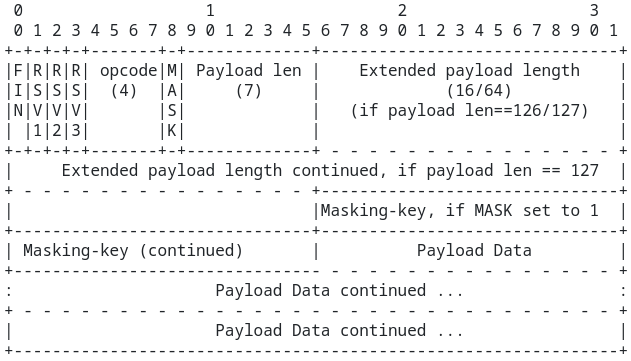
\includegraphics[scale=0.8]{res/ws-frame}
\caption{Фрейм WebSocket протокола}
\end{figure}


Теперь подробнее рассмотрим назначение флагов и возможные значения:
\begin{itemize}
\item \texttt{FIN} -- это 1-битовый флаг, указывающий, является ли обрабатываемый пакет последним фрагментом в сообщении. Значение 0 означает промежуточный пакет, а 1 -- последний пакет. Таким образом, если передаётся длинное сообщение, то 1 будет только у последнего пакета, а если короктое -- то у одного единственного (первого и последнего) пакета.
\item \texttt{RSV (Reserved bits)} -- это 3 битовых флага, отведенный для будущих расширений протокола. RSV1, RSV2 и RSV3 должны иметь значение 0, если они не используются каким-либо расширением.
\item \texttt{OpCode} --это 4-битовый код, определяющий вид полезной нагрузки. Значение OpCode может быть:
\begin{itemize}
	\item \texttt{0x1} обозначает текстовый фрейм.
    \item \texttt{0x2} обозначает двоичный фрейм.
    \item \texttt{0x3} зарезервированы для будущих фреймов с данными.
    \item \texttt{0x4} зарезервированы для будущих фреймов с данными.
    \item \texttt{0x5} зарезервированы для будущих фреймов с данными.
    \item \texttt{0x6} зарезервированы для будущих фреймов с данными.
    \item \texttt{0x7} зарезервированы для будущих фреймов с данными.
    \item \texttt{0x8} обозначает закрытие соединения этим фреймом.
    \item \texttt{0x9} обозначает PING.
    \item \texttt{0xA} обозначает PONG.
    \item \texttt{0xB} зарезервированы для будущих управляющих фреймов.
    \item \texttt{0xC} зарезервированы для будущих управляющих фреймов.
    \item \texttt{0xD} зарезервированы для будущих управляющих фреймов.
    \item \texttt{0xE} зарезервированы для будущих управляющих фреймов.
    \item \texttt{0xF} зарезервированы для будущих управляющих фреймов.
    \item \texttt{0x0} обозначает фрейм-продолжение для фрагментированного сообщения. Он интерпретируется, исходя из ближайшего предыдущего ненулевого типа.
\end{itemize}
\item \texttt{MASK} -- это 1-битовый флаг, указывающий, применяется ли маска к полезной нагрузке. Для всех отправляемых клиентом сообщений \texttt{MASK} должен быть равен 1, а для всех сообщений сервера — равен 0.
\item \texttt{Payload len} -- это поле может занимать 7 битов, 7+16 битов, или 7+64 битов и хранит длинну тела, т.е. размер передаваемых данных.
\begin{itemize}
    \item "0-125" указывает длину полезной нагрузки в октетах;
    \item "126" указывает, что следующие 2 октета интерпретируются как 16-битное беззнаковое целое число, определяющее длину полезной нагрузки;
    \item "127" указывает, что следующие 8 октетов интерпретируются как 64-битное беззнаковое целое число, определяющее длину полезной нагрузки.
\end{itemize}
Эта сложная схема необходима для минимизации издержек: рассмотрим сообщений длиной 125 байт (и менее), тогда для хранения длины потребует всего 7 битов; для больших сообщений (в пределах 65536) -- 7 битов + 2 байта; а для еще ещё больших -- 7 битов и 8 байт. Этого будет достаточно для хранения длины сообщения размером в гигабайт и более.
\item \texttt{Masking-key} -- если флаг \texttt{MASK} установлено 0, то этого полня нет; иначе, это 4-байтное поле содержат маску, которая налагается на тело сообщения.
\item \texttt{Payloat data} -- После заголовка следует полезная нагрузка, которая может включать текстовые или двоичные данные. Маскировка предотвращает возникновение проблем на уровне более низких слоев сетевой инфраструктуры, связанных с неконтролируемым форматом бинарных данных.
\end{itemize}

\subsubsection{Примеры пакетов}

Не фрагментированное текстовое сообщение "Hello" без маски может выглядеть так:

\begin{lstlisting}[style=CommandLineStyle]
0x81 0x05 0x48 0x65 0x6c 0x6c 0x6f
\end{lstlisting}

Состояние флагов будет следующим:
\begin{itemize}
\item \texttt{FIN = 1} -- это короткое сообщение, первый пакет является и последним;
\item \texttt{OpCode = 0x1} -- простой текстовый фрейм.
\end{itemize}

Таким образом, мы получаем \texttt{10000001} в двоичной системе счисления, или \texttt{0x81} в шестнадцатеричной. Полосе заголовка идёт размер длинны тела (\texttt{0x5}) и само тело с текстом.

Фрагментированное текстовое сообщение "Hello", " ", "World" (из трёх частей), без маски может выглядеть так:
\begin{lstlisting}[style=CommandLineStyle]
0x01 0x05 0x48 0x65 0x6c 0x6c 0x6f
0x00 0x01 0x20
0x80 0x05 0x57 0x6f 0x72 0x6c 0x64
\end{lstlisting}

Состояние флагов будет следующим:
\begin{itemize}
\item У первого фрейма \texttt{FIN = 0} и текстовый опкод \texttt{OpCode = 0x1};
\item у второго фрейма \texttt{FIN = 0} и \texttt{OpCode = 0x0} (при фрагментации сообщения, у всех фреймов, кроме первого, опкод пустой);
\item У третьего (завершающего) фрейма \texttt{FIN = 1}.
\end{itemize}

\subsection{WebSocket API}

WebSocket объект обеспечивает API для установки и контроля веб-сокет соединения с сервером, а также для передачи и приема данных через данное соединение. На данный момент полная спецификация поддерживается всеми браузерами \cite{label3}.

Конструктор WebSocket имеет один обязательный параметр и один необязательный параметр:

\begin{lstlisting}[style=CommandLineStyle]
WebSocket WebSocket(
  in DOMString url,
  in optional DOMString protocols
);

WebSocket WebSocket(
  in DOMString url,
  in optional DOMString[] protocols
);
\end{lstlisting}

\begin{itemize}
\item \texttt{url} -- ссылка для подключения; сервер по данному адресу должен откликнуться на запрос websocket.
\item \texttt{protocols} (опционально) -- протокол представлен в виде строки или списка строк протоколов. Эти строки служат для определения клиентских подпротоколов, поскольку один сервер может поддерживать различные WebSocket-подпротоколы (например, чтобы один сервер мог обрабатывать разные виды коммуникаций на основе указанного протокола). Если значение протокола не указано, по умолчанию используется пустая строка.
\end{itemize}

Если порт, на который устанавливается соединение заблокирован, конструктор может выбросить исключение "\texttt{SECURITY\_ERR}".

\subsubsection{Константы состояния готовности}

Константы используются атрибутом \texttt{readyState} для описания состояния WebSocket подключения

\begin{itemize}
\item \texttt{CONNECTING} -- Соединение ещё не открыто.
\item \texttt{OPEN} -- Соединение открыто и готово к обмену данными.
\item \texttt{CLOSING} -- Соединение в процессе закрытия.
\item \texttt{CLOSED} -- Соединение закрыто или не может открыться.
\end{itemize}

\subsubsection{Методы}

\texttt{close()}. Закрывает WebSocket - подключение или заканчивает попытку подключения. Если подключение уже закрыто, этот метод не делает ничего.

\texttt{send()}. Передаёт данные на сервер через WebSocket - соединение.

\section{Сравнение WebSocket с другими технологиями}

\subsection{HTTP-поллинг}


Длинные опросы (long polling) -- это технология, которая была разработана для решения проблемы латентности при использовании обычных опросов (веб-запросов с задержками), вызванных ограничениями стандартных HTTP-соединений. Вместо того чтобы постоянно отправлять новые запросы на сервер для проверки обновлений и тем самым создавать большую нагрузку на сервер, длинный опрос позволяет клиенту отправить один запрос, который будет "держаться" сервером, пока не появится новая информация для отправки клиенту. После отправки этой новой информации сервер закрывает соединение, и клиент немедленно запрашивает новое подключение.

Главным преимуществом длинных опросов является его совместимость с большинством существующих веб-серверов и HTTP-инфраструктуры, что упрощает его интеграцию в уже развернутые системы. Однако, длинные опросы могут столкнуться с ограничениями производительности из-за потребности в постоянной отправке новых запросов и создания новых подключений, что может вызвать задержку при передаче данных. Особенно это заметно при большом количестве активных клиентов.

В то же время, WebSocket обеспечивает более высокую производительность, так как постоянное соединение устраняет задержку и снижает расходы на обработку запросов. Кроме того, WebSocket обеспечивают лучшую поддержку двоичных данных и сжатия, что позволяет сократить объем передаваемых данных и ускорить их обмен. Недостатки WebSocket связанные с поддержкой браузерами уже в прошлом.

В зависимости от конкретного проекта и требований, можно использовать как длинные опросы, так и WebSocket. Если важно сохранение совместимости с существующими клиентами (к примеру, устаревшие версии Android) и инфраструктурой, и потребность в активной связи между клиентом и сервером не является критичной, то можно использовать длинные опросы. Однако, если проект требует быстрой и эффективной передачи данных с минимальными задержками, WebSocket является более оптимальным выбором для реализации взаимодействия между клиентом и сервером.

\subsection{Server-Sent Events (SSE)}

Server-Sent Events (SSE) представляет собой технологию, позволяющую серверу отправлять обновления клиенту через односторонний HTTP-канал без необходимости инициирования новых запросов со стороны клиента. SSE обычно используется для отправки уведомлений или обновлений статуса устройств, что в свою очередь позволяет снизить нагрузку на сервер и повысить скорость обмена данными.

Основное отличие между Server-Sent Events (SSE) и WebSocket состоит в режиме коммуникации. SSE предоставляет только одностороннее подключение (от сервера к клиенту), в то время как WebSocket обеспечивает двустороннее общение. Это означает, что SSE идеально подходит для ситуаций, где серверу необходимо отправлять информацию клиенту, но клиент не обязан отсылать данные серверу. Однако, если клиенту требуется отправить данные серверу, например, для обработки пользовательского ввода, WebSocket будет предпочтительнее.

С точки зрения производительности и надежности, Server-Sent Events и WebSocket можно считать сравнительно равными. Обе технологии обладают низкими задержками и малым оверхедом, что делает их подходящими для использования в интерактивных приложениях. Однако стоит обратить внимание на то, что некоторые функции, доступные в WebSocket, отсутствуют в SSE. К таким функциям относится, например, возможность отправки бинарных данных.

Выбор между Server-Sent Events и WebSocket зависит от конкретных задач, которые ставятся перед разработчиками. SSE подходит для ситуаций с однонаправленным обменом данными, особенно если серверу необходимо отправлять частые обновления клиенту. WebSocket же является идеальным решением для двусторонних взаимодействий и приложений, где важна реакция на пользовательский ввод в режиме реального времени.

\subsection{WebRTC}

Технология WebRTC (Web Real-Time Communications) была разработана для обмена данными в режиме реального времени между двумя браузерами без участия централизованного сервера. Она поддерживает передачу потоковых данных, таких как аудио, видео и единственные наборы данных бинарных и обычных текстовых форм. WebRTC состоит из трех основных API: MediaStream, RTCPeerConnection и RTCDataChannel. Эти API работают совместно, чтобы установить пару pub/sub (поведенческий шаблон проектирования передачи сообщений "Издатель - подписчик") с использованием протоколов SCTP и ICE (включая STUN и TURN). Ключевым аспектом WebRTC является возможность значительно снижать задержку обмена данными и работать в условиях реального времени. Это делает технологию WebRTC чрезвычайно полезной для видео- и аудиоконференций, P2P-игры и других решений, требующих быстрого взаимодействия между участниками.

WebSocket, с другой стороны, представляет собой универсальный протокол для обмена данными между клиентом и сервером, построенный поверх протокола HTTP, который поддерживает инициацию соединения на сервере. WebSocket работает через TCP, что может привести к задержкам из-за перегрузки сети или медленной передачи данных. В отличие от WebRTC, WebSocket требует промежуточного сервера для обработки запросов от клиента, что увеличивает задержки и зависимость от сервера.

Сравнивая технические характеристики, можно отметить, что WebRTC имеет больше возможностей, включая адаптивное кодирование, снижение задержки и аппаратные возможности ускорения через GPU. WebSocket имеет более простую структуру, что облегчает развертывание и снижает нагрузку на сервер. Однако необходимость использования серверов делает WebSocket более затратной технологией по сравнению с децентрализованным подходом WebRTC.

В итоге можно сказать, что WebRTC и WebSocket представляют разные классы технологий, каждая из которых имеет свои достоинства и недостатки. WebRTC подходит для видеочатов, тогда как WebSocket решает проблему обмена сообщениями. В некоторых ситуациях возможно использование обеих технологий в одной системе, с учетом уникальных преимуществ каждой из них.
\chapter{Реализация клиент-серверного взаимодействия по протоколу WebSocket}

\section{Пример простого чата (node.js)}

Рассмотрим пример приложения, созданного на node.js.

Сервер запускается на порту 8080, и ожидает подключения клиента (листинг 2.1). В данном случае мы не обеспечиваем никакого шифрования и должной обработки ошибок, наша задача просто продемонстрировать принцип работы.

\lstinputlisting[language=JavaScript, caption={Исходный код сервера node.js приложения}]
{example1/server.js}

Как только клиент подключился, сервер отдаёт ему HTML страницу с кодом на JavaScript. Этот выполняет WebSocket подключение к серверу для обмена сообщениями (листинг 2.2).

\lstinputlisting[language=HTML, caption={Исходный код клиента}]
{example1/index.html}

Если открыть это соединение из двух разных браузеров, можно устроить простой чат (рисунок 2.1).

\begin{figure}[H]
\centering
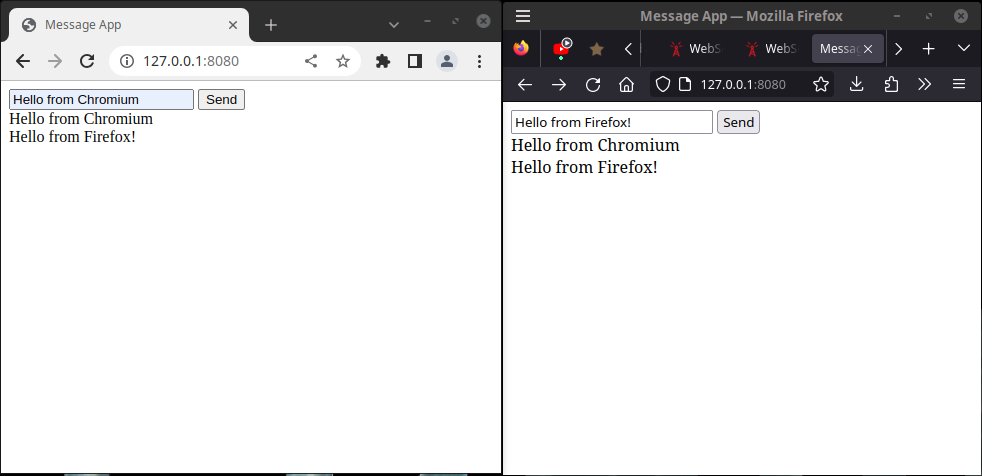
\includegraphics[scale=0.5]{res/browsers1}
\caption{Взаимодействие между двумя разными браузерами}
\end{figure}

В это время в терминале можно видеть сообщения, которыми обмениваются клиенты (рисунок 2.2).

\begin{figure}[H]
\centering
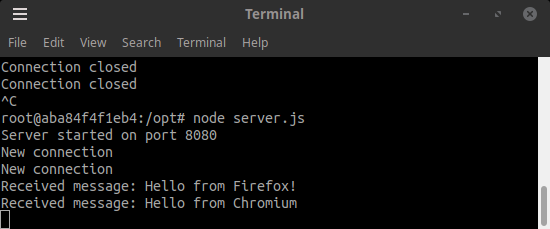
\includegraphics[scale=1]{res/console1}
\caption{Консоль серверного приложения}
\end{figure}

\section{Пример тестера скорости соединения (Rust)}

Второй пример представляет из себя немного более сложный код. Идея проекта в том, чтобы передать через WebSocket соединение файл объёмом 10 мб и замерить скорость передачи.

Сервер так же запускается на порту 8080 (листинг 2.3), и готов отдать пользователю статичный HTML файл.

\lstinputlisting[language=Rust, caption={Исходный код сервера Rust приложения}]
{example2/src/main.rs}

Управление раутами и временем жизни соединения в этот раз вынесено в отдельный файл (листинг 2.4)

\lstinputlisting[language=Rust, caption={Управление WebSocket соединением}]
{example2/src/server.rs}

Клиентское приложение представляет из себя HTML страницу (листинг 2.5). Её код тривиален, поэтому в листинге обратим внимание только на JavaScript код.

\lstinputlisting[language=JavaScript, caption={Исходный код сервера node.js приложения}, , firstline=83, lastline=175]
{example2/static/index.html}

В панели веб-разработчика можно видеть, что файл действительно был передан именно через WebSocket (рисунок 2.3).

\begin{figure}[H]
\centering
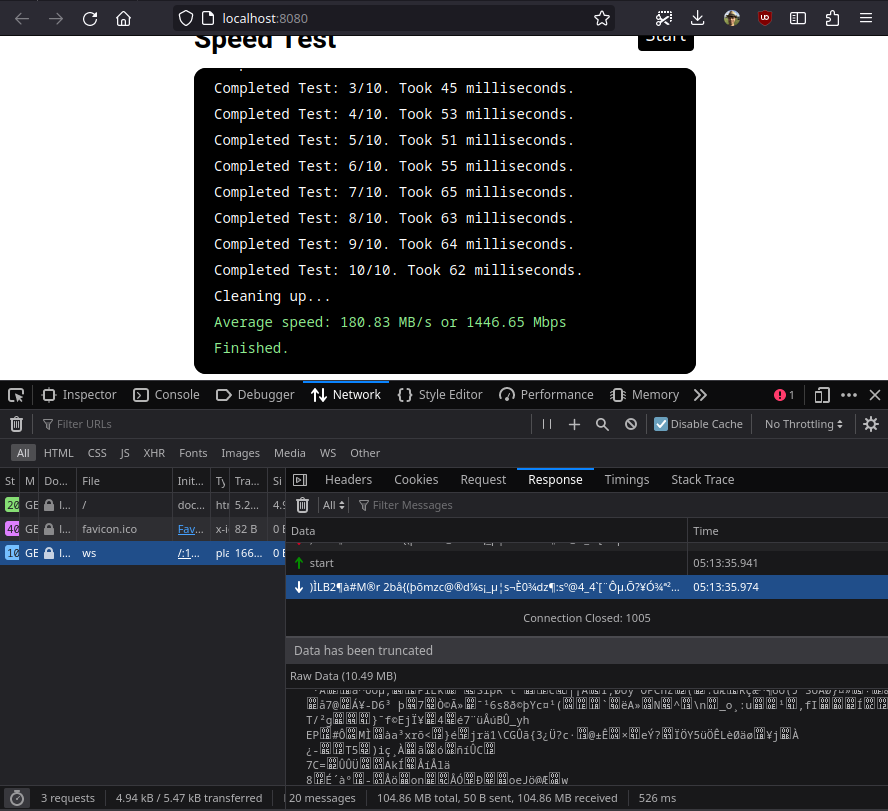
\includegraphics[scale=0.6]{res/browser2}
\caption{Панель веб-разработчика}
\end{figure}

\chapter{Применение WebSocket в Web-среде}

Использование WebSocket на производственных серверах в условиях реального веба требует повышенного внимания к безопасности и производительности.

\section{Безопасность WebSocket}

Хотя WebSockets предлагают мощное средство для разработки приложений коммуникации в реальном времени, они также создают определенные угрозы безопасности, которые следует принимать во внимание. Вот некоторые распространенные проблемы безопасности, связанные с WebSockets, а также стратегии их устранения:

Перехват WebSocket между сайтами (CSWSH): возникает, когда злоумышленник использует уязвимость XSS для кражи соединения WebSocket и связи с сервером. Для предотвращения этого, разработчику важно убедиться, что соединение WebSocket устанавливается исключительно между доверенными сторонами. Внедрение аутентификации на стороне сервера поможет предотвратить такие атаки.

Подделка межсайтовых запросов (CSRF): возникает, когда злоумышленник отправляет запрос WebSocket на сервер от имени другого пользователя. Для предотвращения этого, важно использовать CSRF-токены, чтобы обеспечить прием запроса WebSocket только от доверенных источников.

Инъекционные атаки: они возникают, когда злоумышленник внедряет вредоносный код или данные в запрос или ответ WebSocket. Для предотвращения атак с использованием инъекций, важно скрупулезно проверять и фильтровать все данные, отправляемые через соединение WebSocket. Реализация проверки входящих данных и кодирования исходящих данных может помочь избежать инъекционных атак.

Атаки "отказ в обслуживании" (DoS): возникают, когда злоумышленник перегружает сервер большим числом запросов WebSocket, что может привести к сбою сервера. Для предотвращения DoS-атак важно внедрить ограничение скорости и дросселирование, чтобы снизить количество запросов, которые сервер способен обрабатывать.

Атаки "человек посередине" (MitM): возникают, когда злоумышленник перехватывает трафик WebSocket и просматривает или изменяет данные, передаваемые между клиентом и сервером. Чтобы предотвратить атаки MitM, важно внедрить меры шифрования и аутентификации, такие как SSL/TLS, чтобы обеспечить безопасность трафика WebSocket и защиту от перехвата или изменения.

В общем, важно надлежащим образом обезопасить соединение WebSocket, внедряя такие меры, как проверка вхождений, кодирование выходных данных, аутентификация, шифрование, ограничение скорости и CSRF-токены. Следуя рекомендациям по обеспечению безопасности WebSocket, разработчики смогут предотвратить типичные проблемы безопасности и обеспечить надежность и безопасность их приложений для обмена данными в реальном времени.

\subsection{Шифрование и обеспечение конфиденциальности}

Протокол WebSocket поддерживается практически всеми современными браузерами включая Chrome, Firefox, Internet Explorer, Opera, и Safari. Однако по спецификации, этот протокол не обеспечивает шифрования, а значит может быть перехвачен, прочитан и даже изменён. Поскольку WebSocket это централизованный протокол (т.е. предполагает наличие сервера) то проблему защиты данных нужно решать на стороне серверных платформ начинает поддерживать этот протокол.

NGINX с одной стороны умеет терминировать SSL/TLS траффик, с другой -- поддерживает WebSocket, позволяя установить туннель между клиентом и сервером бэкэнда\cite{label4}. Чтобы NGINX отправил запрос на обновление от клиента к серверу бэкэнда, заголовки Upgrade и Connection должны быть установлены явно, как в этом примере:

\begin{lstlisting}[style=CommandLineStyle]
location /wsapp/ {
    proxy_pass http://wsbackend;
    proxy_http_version 1.1;
    proxy_set_header Upgrade $http_upgrade;
    proxy_set_header Connection "Upgrade";
    proxy_set_header Host $host;
}
\end{lstlisting}

После этого NGINX обрабатывает это как соединение WebSocket.

\subsection{Атака ``отравленный кэш``}

В ранних реализациях WebSocket существовала уязвимость, известная как «cache poisoning» (отравленный кэш)\cite{label1}. Эта уязвимость позволяла атаковать кэширующие прокси-серверы, особенно корпоративные системы.

Атака выполнялась следующим образом:
\begin{enumerate}
\item Злоумышленник привлекает доверчивого пользователя (далее - Жертва) на свой сайт.
\item На сайте Злоумышленника, веб-страница открывает WebSocket-соединение из браузера Жертвы к серверу Злоумышленника. Предполагается, что жертва использует прокси-сервер, который является целью атаки.
\item Веб-страница создает особый WebSocket-запрос, который некоторые прокси-сервера не могут распознать (и в этом есть условие для успешной атаки).
\item Прокси-сервер Жертвы пропускают начальный запрос (содержащий Connection: upgrade) и полагает, что следующий HTTP-запрос уже поступил. Однако на самом деле вместо этого данные передаются через WebSocket! Обе стороны WebSocket (веб-страница и сервер) контролируются Злоумышленником!
\item Злоумышленник может передать что-то, похожее на GET-запрос к известному ресурсу, например: http://code.jquery.com/jquery.js. Тогда сервер ответит, имитируя код jQuery с кэширующими заголовками. Прокси-сервер получит этот ответ и закэширует искажённую версию jQuery.
\item В результате, при загрузке новых страниц, другие пользователи, использующие тот же прокси-сервер, что и Жертва, получат хакерский код вместо настоящего jQuery (это и объясняет название атаки - «отравленный кэш».).
\end{enumerate}

Эта атака не работает для всех прокси-серверов, однако при исследовании уязвимости было доказано, что реальные уязвимые прокси-серверы существуют. 

Для предотвращения такой атаки разработали метод защиты - использование «маски».

\subsubsection{Маска для защиты от атаки}

Маска, которую мы рассматривали ранее при изучении полей WebSocket пакета, создана для предотвращения атаки отравленного кэша. 

Ключ маски -- это случайное 32-битное значение, которое меняется для каждого пакета данных.

Тело сообщения проходит через \texttt{XOR} $\oplus$ с маской, а получатель восстанавливает данные, применяя повторно \texttt{XOR} с маской (можно легко доказать, что $(x \oplus a) \oplus a == x$).

Маска служит двум целям:
\begin{enumerate}
\item Генерируется браузером. Таким образом, злоумышленник больше не может контролировать реальное содержимое тела сообщения. После наложения маски данные превращаются в бинарный беспорядок.
\item Полученный пакет данных уже не может быть воспринят промежуточным прокси как HTTP-запрос.
\end{enumerate}

Наложение маски требует дополнительных ресурсов, поэтому в протоколе WebSocket оно не является обязательным.

Если используется два клиента (не обязательно браузеры), которые доверяют друг другу и посредникам, можно установить бит маски в 0, и тогда не потребуется указывать ключ маски.

\section{Производительность и масштабируемость}

Когда речь заходит о промышленном применении и высоких нагрузках, встаёт вопрос масштабируемости.

\subsubsection{Вертикальное и горизонтальное масштабирование}

Первый тип - вертикальное масштабирование, что является простым путем увеличения производительности приложения, хотя и имеет свои ограничения. Это, в перву очередь, ресурсы: берётся один экземпляр приложения и улучшаем аппаратное обеспечение (процессор, объем памяти, ввод-вывод и т.д.). Этот метод не требует дополнительных затрат с точки зрения разработки, однако не является самым эффективным для масштабирования.

Главным недостатком вертикального масштабирования является то, что время исполнения кода не изменяется линейно с улучшением оборудования. Кроме того, существует ограничение на возможности аппаратных усовершенствований - нет возможности неограниченно повышать производительность процессора.

Значит, есть другая альтернатива - горизонтальное масштабирование, которое предполагает создание дополнительных экземпляров приложения вместо добавления ресурсов к существующим. Это позволяет практически неограниченно масштабировать систему с возможностью динамического масштабирования при изменении нагрузок.

С точки зрения разработки, у нас появляется дополнительный элемент в системе -- балансировщик нагрузки. А в некоторых случаях, придётся внести изменения в архитектуру, добавив реализацию pub/sub.

\subsubsection{Проблема состояния и липкая сессия}

Простые REST API сервера не хранят состояние. И горизонтальное масштабирование для таких серверов превращается в тривиальную задачу: мы можем случайным образом раскидывать запросы клиентов, и нам не важно какой экземпляр приложения этот запрос обработает.

Вот так может выглядеть конфиг для балансировщика HAProxy \cite{label5}

\begin{lstlisting}[style=CommandLineStyle]
defaults
  mode http
  option http-server-close
  timeout connect     5s
  timeout client      30s
  timeout client-fin  30s
  timeout server      30s
  timeout tunnel      1h
  default-server inter 1s rise 2 fall 1 on-marked-down shutdown-sessions
  option forwardfor

frontend all
  bind 127.0.0.1:8080
  default_backend backends

backend backends
  server srv1 127.0.0.1:8081 check
  server srv2 127.0.0.1:8082 check
\end{lstlisting}

с WebSocket ситуация иначе, так как каждое сокетное соединение привязано к определенному экземпляру. В таком случае, нужно гарантировать, что все запросы отдельных пользователей направляются к нужному бэкэнду. 

Для решения этой проблемы можно использовать липкие сессии. Балансировщик нагрузки HAProxy вместо циклического перебора будет использовать стратегию с минимальным количеством подключений и добавим куки для привязки запросов пользователей к определенному бэкэнду. Тогда запрос от одного пользователя будет приходить всегда на один и тот же сервер.

\begin{lstlisting}[style=CommandLineStyle]
backend backends
  balance leastconn
  cookie serverid insert
  server srv1 127.0.0.1:8081 check cookie srv1
  server srv2 127.0.0.1:8082 check cookie srv2
\end{lstlisting}

\subsubsection{Рассылка широковещательных сообщений}

Предположим, что возникает необходимость отправить сообщение сразу всем пользователям системы. Либо пользователи подписаны на один канал, при этом подключены к разным физическим серверам. Очевидно, что решить эту задачу в рамках одного сервера невозможно, т.к. он просто не знает о всех пользователях.

Решение этой задачи заключается в организации связи между разными экземплярами приложения на разных серверах. Для этого все экземпляры могут быть подписаны на определенный канал и обрабатывать входящие сообщения. Это применение паттерна pub/sub о котором мы уже говорили ранее. Существует большое количество готовых продуктов подобного рода, таких как Redis, Kafka или Nats.
\chapter*{Заключение}
\addcontentsline{toc}{chapter}{Заключение}

В ходе проведенного исследования были рассмотрены основные возможности протокола WebSocket, его устройство и приведены практические примеры использования. Целью работы было изучить протокол WebSocket и понять его преимущества и особенности по сравнению с другими технологиями для обмена данными в режиме реального времени.

Основные принципы WebSocket, такие как двунаправленная связь, инициация соединения сервером, поддержка реального времени, эффективное использование ресурсов и совместимость с прокси-серверами и брандмауэрами, делают его идеальным выбором для приложений, требующих непрерывного обмена данными между клиентом и сервером.

Архитектура WebSocket, включающая установку и завершение соединения, фреймы и их структуру, а также WebSocket API, предоставляет гибкую платформу для разработки приложений реального времени. Протокол WebSocket также был сравнен с другими технологиями, такими как HTTP-поллинг, Server-Sent Events (SSE) и WebRTC, и показал высокий уровень в области производительности и эффективности.

В работе были представлены практические примеры использования WebSocket, включая реализацию простого чата на платформе node.js и создание тестера скорости соединения на языке программирования Rust. Эти примеры демонстрируют, как легко и эффективно можно использовать протокол WebSocket для различных типов приложений.

Выводы по работе:
\begin{enumerate}
\item Протокол WebSocket - полезная и востребованная технология для реализации обмена данными между клиентом и сервером в режиме реального времени. Это достигается благодаря двунаправленной связи, низкому времени задержки и эффективному использованию ресурсов.
\item WebSocket обладает рядом преимуществ перед другими технологиями, что делает его актуальным выбором для решения задач, связанных с обменом данными в режиме реального времени.
\item Несмотря на свои преимущества, важно учесть возможные риски, связанные с безопасностью и производительностью при использовании WebSocket в конкретном проекте, и применить соответствующие меры для смягчения этих рисков.
\item Практические примеры использования WebSocket успешно применяются для решения различных задач, свидетельствующих об универсальности и вариативности этой технологии.
\end{enumerate}

Таким образом, в результате исследования и анализа данного протокола можно сделать вывод о его значимости для обеспечения непрерывного и эффективного обмена данными в режиме реального времени. Его преимущества, такие как низкая задержка, масштабируемость, поддержка расширений и простота использования, делают его идеальным выбором для разработки современных веб-приложений. Протокол WebSocket открывает новые возможности в области интерактивных веб-приложений, многопользовательских игр, финансовых торговых платформ и других приложений, где важна своевременная доставка данных и низкая задержка взаимодействия.
% \newpage
\section*{}
\addcontentsline{toc}{section}{List of sources}

\begin{thebibliography}{00}

% Use: \cite{label1}
\bibitem{label1} JavaScript.ru: Справочник по работе с WebSocket. URL: https://learn.javascript.ru/websockets (дата обращения: 16.04.2023).

\bibitem{label2} Internet Engineering Task Force (IETF) / Request for Comments: 6455: The WebSocket Protocol (December 2011). URL: https://datatracker.ietf.org/doc/html/rfc6455 (дата обращения: 20.04.2023).

\bibitem{label3} MDN Web Docs / The WebSocket API (WebSockets). URL: https://developer.mozilla.org/en-US/docs/Web/API/WebSockets\_API (дата обращения: 20.04.2023).

\bibitem{label4} Nginx blog / NGINX as a WebSocket Proxy (Rick Nelson, 2014). URL: https://www.nginx.com/blog/websocket-nginx/ (дата обращения: 23.04.2023).

\bibitem{label5} How to scale WebSocket – horizontal scaling with WebSocket tutorial (2020). URL: https://tsh.io/blog/how-to-scale-websocket/ (дата обращения: 26.04.2023).

\end{thebibliography}                              % inclide the list of sources


\end{document}

%------------------------------------------------------------------------------
% Examples:
%
%
% Image:
% \begin{figure}[H]
% \centering
% \includegraphics[scale=0.8]{res/pic01}
% \caption{Picture description}
% \end{figure}
%
%
% Table:
% \begin{table}[htb]
%     \begin{tabularx}{\textwidth}{|X|c|c|c|c|c|}
%     \hline
%     \multirow{2}{*}{tb1} & \multirow{2}{*}{tbl2} & \multicolumn{4}{c|}{tbl3} \\
%     \cline{3-6}
%     {} & {} & A & B & C & D\\
%     \hline
%     Text & {} & Text & {} & {} & {} \\
%     \hline
%     \end{tabularx}
% \caption{Table description}
% \end{table}
%
% Something in a frame:
% \begin{Verbatim}[frame=single,breaklines=true,breakanywhere=true]
%    user@ubuntu$ cat /proc/sys/fs/file-nr
% \end{Verbatim}
%
%
% CPP code
% \lstinputlisting[language=C++, caption={Фрагмент исходного кода модифицированного файла игры}, firstline=73, lastline=80]
% {../Tasks/2_L4_Socket_sample/source_files/server_game_upd.cpp}
%
%
% Any other code
% \fbox{
%     \parbox{\textwidth}{%
%     \texttt{\noindent
%     \#<domain>      <type>  <item>         <value>\\
%     oracle          hard    nofile         8192
%     }}%
% }
%
%
% Console output
% \begin{lstlisting}[style=CommandLineStyle]
%     user@ubuntu$ sudo sysctl fs.file-max=65536
%     [sudo] password for user: 
%     fs.file-max = 65536
% \end{lstlisting}
%
%
% Color box
% \fbox{
%     \parbox{\textwidth}{%
%     \texttt{\noindent
% 0000|   \hl{14 5a fc 0d 56 2d} 34 ce 00 37 d9 03 08 00 45 00\\
% 0010|   00 54 20 30 00 00 40 01 e0 e8 c0 a8 7c 01 c0 a8\\
% 0020|   7c 3e 00 00 d3 bd 00 02 00 0e 7a c1 e8 63 00 00\\
% 0030|   00 00 08 3a 02 00 00 00 00 00 10 11 12 13 14 15\\
% 0040|   16 17 18 19 1a 1b 1c 1d 1e 1f 20 21 22 23 24 25\\
% 0050|   26 27 28 29 2a 2b 2c 2d 2e 2f 30 31 32 33 34 35\\
% 0060|   36 37
%     }}%
% }
%